\chapter{Resultados e Discussão}
\label{chap:resultados}

Neste capítulo, trazemos os achados e a análise dos mesmos utilizando a ARS e do discurso dos entrevistados, ressaltando aos temas que se sobressaíram nas entrevistas. As respostas foram fornecidas objetivando vislumbrar a caracterização e o funcionamento desta rede para pacientes hipertensos e diabéticos. 

\section{Análise da Rede Social: o enfermeiro ocupando espaços de destaque no sistema de saúde}

Analisar redes sociais permite vislumbrar as interações entre qualquer classe de indivíduos, partindo tanto de dados qualitativos quanto quantitativos. Segundo \cite{stanley1994social},  o uso de  análise de redes sociais possibilita coletar informações relevantes sobre a estrutura de um grupo, sendo possível, identificar as posições ocupadas pelos indivíduos, bem como identificar o cerne das relações criadas ao redor de cada um.

Como explicado anteriormente, os dados foram coletados no município de Icapuí-Ce, na \acrlong{UBS} da localidade de Barreira assim como em outros locais (Secretaria de Saúde do Município, o Centro de Atenção Psicossocial e o Hospital Municipal Maria Idalina Rodrigues de Medeiros), considerando as pessoas citadas nas entrevistas.

Logicamente, uma infinidade de análises pode ser realizada considerando os dados coletados, o que pode ser inviável de abordar em um único trabalho. Portanto, um número limitado de atores, conexões e métricas foi utilizado, e a partir deles, foram feitas considerações sobre o comportamento geral da rede social de uma única enfermeira. 

A rede pesquisada não contempla todas as relações possíveis e existentes de cada pessoa entrevistada, mas somente um recorte viável de analisar. As notações consideradas no desenho do grafo estão reunidas nas tabelas \ref{graph-job} e \ref{graph-place}.

\begin{table}[htbp]
\centering
\caption{Significado dos rótulos dos atores da rede segundo suas profissões.}
\label{graph-job}
\begin{tabular}{|l|l|}
\hline
Notação  & Profissão               \\ \hline
E        & Enfermeiro(a)           \\ \hline
E{[}R{]} & Enfermeiro(a) Residente \\ \hline
F        & Farmacêutico(a)         \\ \hline
N        & Nutricionista           \\ \hline
N{[}R{]} & Nutricionista Residente \\ \hline
M        & Médico(a)               \\ \hline
A        & Outro                   \\ \hline
\end{tabular}
\end{table}

\begin{table}[htbp]
\centering
\caption{Significado dos rótulos dos atores da rede segundo as áreas de atuação.}
\label{graph-place}
\begin{tabular}{|l|l|}
\hline
Notação & Área de Atuação                       \\ \hline
{[}H{]} & Hospital                      \\ \hline
{[}S{]} & Secretaria de Saúde de Icapuí \\ \hline
{[}P{]} & Policlínica de Aracati        \\ \hline
        & Atenção Básica                \\ \hline
\end{tabular}
\end{table}

Além disso, a identificação dos atores segue a seguinte notação [Profissão][Identificador Único] [Área de Atuação], por exemplo, $E1 [R]$ (Enfermeiro(a) 01 Residente); $E2$ (Enfermeiro 02 Atenção básica) etc.

Como pode ser observado na Figura \ref{fig:grafos}, o grafo permite identificar vinte e seis (26) atores que fazem parte da rede, onde seis (6) pessoas foram entrevistadas, vinte (20) outras foram citadas, trinta (30) relações e nenhum laço.

\begin{figure}[htbp]
\centering
 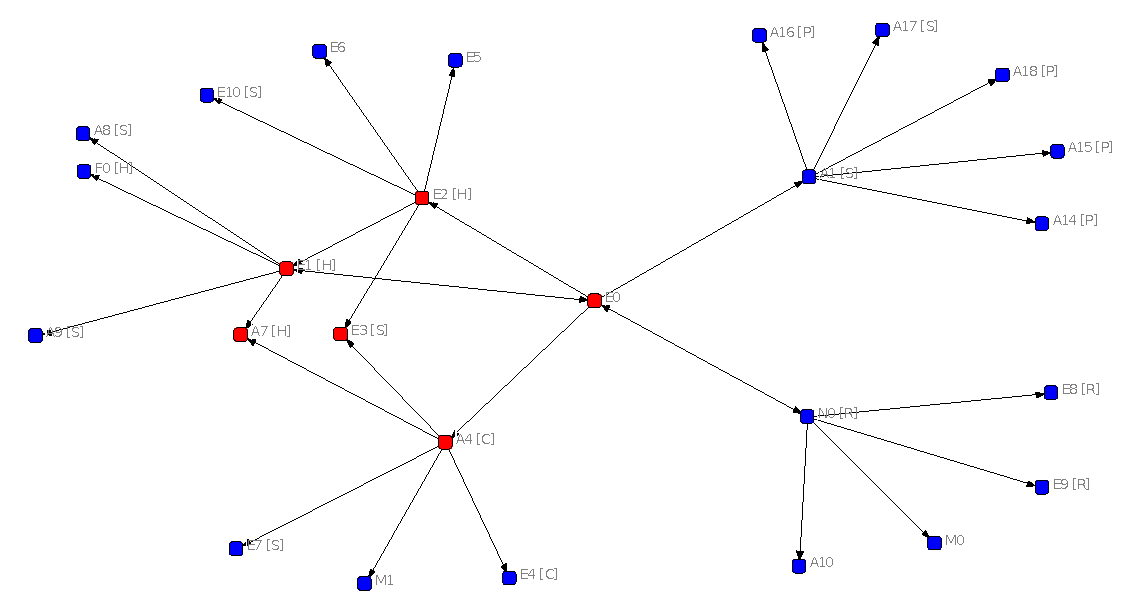
\includegraphics[width=.85\textwidth]{figuras/grafo-grupos.pdf}
 \caption{Representação da rede social utilizada neste trabalho.}
\label{fig:grafos}
\end{figure}

A primeira medida analisada da rede foi a densidade que é a relação entre o número de laços existentes e o número de laços possíveis. Tal métrica exibe a taxa de conectividade da rede. Neste trabalho, o valor de densidade encontrado foi de 4,61\% (baixa densidade) o que pode denotar a existência de alguma dificuldade na resolução de problemas em grupo.

Geralmente, nas circunstâncias onde existe baixa densidade, os atores não conseguem se identificar como participantes de um grupo maior e podem demonstrar certa dificuldade de relacionamento. Tal situação pode acarretar pouca cooperatividade entres os atores envolvidos, podendo até mesmo existir apatia na resolução de problemas, gerando conflitos. \cite{hanneman2001centralidad}.

Entretanto, devemos ressaltar que os atores identificados na rede localizam-se em diferentes espaços de trabalho, o que pode contribuir para uma comunicação mais limitada junto a outros possíveis atores. Além deste fato, as motivações de cada um dos entrevistados na denominação dos atores de suas redes, bem como o número de entrevistados devem ser levados em conta nesta análise como um fator interveniente na densidade. 

Outra medida importante é o grau de centralidade, ele indica o número de ligações que entram e que saem de um ator. Através dele são identificados os atores principais da rede. A tabela \ref{table-centralize-degree} exibe o grau de centralidade associado a cada ator.

\begin{table}[htbp]
\centering
\caption{Grau de centralização de cada ator.}
\label{table-centralize-degree}
\begin{tabular}{|l|l|l|l|l|}
\hline
Identificador & Grau de Saída & Grau de Entrada & Grau de Saída  & Grau de Entrada \\ 
	      &               &                 & Normalizada    & Normalizada \\ \hline
E0            & 5,000         & 2,000           & 0,200                     & 0,080                       \\ \hline
A1 {[}S{]}    & 5,000         & 1,000           & 0,200                     & 0,040                       \\ \hline
E1 {[}H{]}    & 5,000         & 2,000           & 0,200                     & 0,080                       \\ \hline
N0 {[}R{]}    & 5,000         & 1,000           & 0,200                     & 0,040                       \\ \hline
A4 {[}C{]}    & 5,000         & 1,000           & 0,200                     & 0,040                       \\ \hline
E2 {[}H{]}    & 5,000         & 1,000           & 0,200                     & 0,040                       \\ \hline
F0 {[}H{]}    & 0,000         & 1,000           & 0,000                     & 0,040                       \\ \hline
A7 {[}H{]}    & 0,000         & 2,000           & 0,000                     & 0,080                       \\ \hline
A8 {[}S{]}    & 0,000         & 1,000           & 0,000                     & 0,040                       \\ \hline
A9 {[}S{]}    & 0,000         & 1,000           & 0,000                     & 0,040                       \\ \hline
A10           & 0,000         & 1,000           & 0,000                     & 0,040                       \\ \hline
E9 {[}R{]}    & 0,000         & 1,000           & 0,000                     & 0,040                       \\ \hline
E8 {[}R{]}    & 0,000         & 1,000           & 0,000                     & 0,040                       \\ \hline
M0            & 0,000         & 1,000           & 0,000                     & 0,040                       \\ \hline
A14 {[}P{]}   & 0,000         & 1,000           & 0,000                     & 0,040                       \\ \hline
A15 {[}P{]}   & 0,000         & 1,000           & 0,000                     & 0,040                       \\ \hline
A16 {[}P{]}   & 0,000         & 1,000           & 0,000                     & 0,040                       \\ \hline
A17 {[}S{]}   & 0,000         & 1,000           & 0,000                     & 0,040                       \\ \hline
A18 {[}P{]}   & 0,000         & 1,000           & 0,000                     & 0,040                       \\ \hline
E10 {[}S{]}   & 0,000         & 1,000           & 0,000                     & 0,040                       \\ \hline
E3 {[}S{]}    & 0,000         & 2,000           & 0,000                     & 0,080                       \\ \hline
E6            & 0,000         & 1,000           & 0,000                     & 0,040                       \\ \hline
E5            & 0,000         & 1,000           & 0,000                     & 0,040                       \\ \hline
E4 {[}C{]}    & 0,000         & 1,000           & 0,000                     & 0,040                       \\ \hline
M1            & 0,000         & 1,000           & 0,000                     & 0,040                       \\ \hline
E7 {[}S{]}    & 0,000         & 1,000           & 0,000                     & 0,040                       \\ \hline
\end{tabular}
\end{table}

Através da tabela \ref{table-centralize-degree} identifica-se que os principais atores da rede são $E0$, $E1[H]$, $A7 [H]$ e  $E3[S]$ pois cada um possui Grau de Entrada Normalizada de 0,8 (mais requisitados).

$E0$ trata-se de uma enfermeira bastante conhecida no município, pois foi uma das primeiras enfermeiras a integrar a ESF quando esta foi implantada em Icapuí e ainda recebia a denominação de \acrlong{PSF} (\acrshort{PSF}). Está no quadro de funcionários do município como enfermeira desde o fim da graduação tendo passado também pelo Hospital Municipal, integrando a equipe assistencial. Em sua fala, $E0$ coloca que: 

\begin{citacao}
``Esse mesmo tempo, que quando eu me formei eu vim pra cá, e fiquei trabalhando aqui em Barreiras e mais em outra área, a gente conjugava duas unidade de saúde, quando iniciou a formação do PSF do município, então não tinha muito profissional na época, então a gente se dividia em duas equipes, com o passar do tempo que a gente foi... Eu to aqui só em Barreiras mesmo, esses vinte anos, mas eu sempre dividi até o ano passado dividi com outra unidade de saúde.''
\end{citacao}

Por esse longo período imersa na comunidade, inclusive em duas equipes, pela carência de profissionais na época, $E0$ teve a oportunidade de servir como referência a outros profissionais que adentraram no programa posteriormente. Seu período como plantonista no hospital, também proporcionou a ela o desenvolvimento de outras relações com outros profissionais, como $E1 [H]$ e $E2 [H]$.

$E1[H]$ é coordenador do serviço de enfermagem do hospital, além de enfermeiro plantonista. Adentrou no serviço de saúde do município exercendo o cargo de auxiliar de serviços gerais em 1990. A partir daí, fez cursos técnicos tanto na área de enfermagem como na área de análises clínicas, trabalhando na instituição tanto como técnico e auxiliar de enfermagem como técnico em radiologia por seis (6) anos. Graduou-se em Ciências Biológicas e em Enfermagem no ano de 2013. Exercendo atualmente as funções assistenciais e gerenciais na instituição.

$E1[H]$ cita $E0$ e é citado por esta, pois desenvolveram um vínculo devido ao período em que trabalharam juntos no hospital. $E1[H]$ chegou a se emocionar durante a entrevista ao falar de $E0$, denotando o desenvolvimento também de vínculo emocional. Ao citar $A7[H]$, $E1[H]$ apontou a importância do contato baseado nas questões gerenciais, pois $A7[H]$, enquanto diretora administrativa do hospital, conseguia resolver as questões que $E1[H]$ não conseguia dar seguimento.

$A7[H]$ também é apontada por $A4[C]$, técnica de enfermagem e atualmente recepcionista do \acrshort{CAPS} do município, por questões similares, pois os pacientes do CAPS recebem seus medicamentos no hospital, encontrando lá suporte também para outras demandas. 

$E3[S]$ é enfermeiro e atualmente coordena a Atenção Básica. É citado por $A4[C]$ e por $E2[H]$. Estando em um cargo de gestão no município, entra em contato com diferentes profissionais e lida com diversas demandas. É apontado pelos entrevistados que o citaram como alguém sempre acessível e bem próximo a comunidade, conseguindo realizar pactuações e articulações.

Percebemos assim o importante papel que os profissionais de Enfermagem exercem na rede de atenção municipal, ocupando os diferentes espaços não apenas nos níveis de atenção, mas também em funções administrativas e de gestão de recursos. 

O Grau de Proximidade denota a capacidade de um ator se ligar a todos os outros atores de uma rede, ou seja, quanto menor a distância entre um ator e outro, maior será seu grau de proximidade. 

Já o Grau de Intermediação mostra a capacidade que um ator possui de intermediar a comunicação entre pares de atores da rede. Sua importância se dá, pois, através de atores que possuem alto grau de intermediação que as informações são propagadas para diversos outros atores. 

A tabela \ref{closeness-betweeness-degree} lista o Grau de Proximidade e Intermediação dos atores.

\begin{table}[htbp]
\centering
\caption{Grau de Proximidade e Intermediação dos Nós.}
\label{closeness-betweeness-degree}
\begin{tabular}{|l|l|l|}
\hline
Identificador & Grau de Proximidade & Grau de Intermediação \\ \hline
E0            & 55.556              & 66.667                \\ \hline
A1 {[}S{]}    & 42.373              & 36.667                \\ \hline
E1 {[}H{]}    & 44.643              & 26.333                \\ \hline
N0 {[}R{]}    & 40.984              & 30.000                \\ \hline
A4 {[}C{]}    & 42.373              & 27.333                \\ \hline
E2 {[}H{]}    & 44.643              & 26.333                \\ \hline
F0 {[}H{]}    & 31.250              & 0.000                 \\ \hline
A7 {[}H{]}    & 35.211              & 2.667                 \\ \hline
A8 {[}S{]}    & 31.250              & 0.000                 \\ \hline
A9 {[}S{]}    & 31.250              & 0.000                 \\ \hline
A10           & 29.412              & 0.000                 \\ \hline
E9 {[}R{]}    & 29.412              & 0.000                 \\ \hline
E8 {[}R{]}    & 29.412              & 0.000                 \\ \hline
M0            & 29.412              & 0.000                 \\ \hline
A14 {[}P{]}   & 30.120              & 0.000                 \\ \hline
A15 {[}P{]}   & 30.120              & 0.000                 \\ \hline
A16 {[}P{]}   & 30.120              & 0.000                 \\ \hline
A17 {[}S{]}   & 30.120              & 0.000                 \\ \hline
A18 {[}P{]}   & 30.120              & 0.000                 \\ \hline
E10 {[}S{]}   & 31.250              & 0.000                 \\ \hline
E3 {[}S{]}    & 35.211              & 2.667                 \\ \hline
E6            & 31.250              & 0.000                 \\ \hline
E5            & 31.250              & 0.000                 \\ \hline
E4 {[}C{]}    & 30.120              & 0.000                 \\ \hline
M1            & 30.120              & 0.000                 \\ \hline
E7 {[}S{]}    & 30.120              & 0.000                 \\ \hline
\end{tabular}
\end{table}

A partir da tabela \ref{closeness-betweeness-degree} observa-se que os atores $E0$, $A1 [S]$, $E1 [H]$, $N0 [R]$, $A4 [C]$ e $E2 [H]$ possuem os maiores Graus de Proximidade e os atores $E0$, $A1 [S]$ e $N0 [R]$ possuem maiores Graus de Intermediação.

Nesta análise $E0$ possui maior grau de intermediação pois a rede foi construída a partir dela. Mas destaca-se a mesma medida de $A1[S]$. $A1[S]$ é responsável pela distribuição de um grande número de informações na rede. Ela possibilita o acesso a outros profissionais e serviços contactando outros atores, uma vez que encontra-se na Central de Marcação de Consultas do município, realizando o contato da rede municipal de Icapuí com a rede de Aracati através da policlínica.

Com as análises do grafo formado, temos uma visão da importância do enfermeiro na rede, desempenhando a comunicação com diferentes serviços em diferentes espaços de trabalho. Devemos atentar também para a importância da Residência Multiprofissional no município, uma vez que alguns profissionais residentes foram citados. A comunicação aparece bem vinculada aos enfermeiros e aos demais profissionais da enfermagem no grafo, mostrando uma necessidade de envolvimento de outros trabalhadores da saúde no processo.